\section{Nghiên cứu loại trừ}

\subsection{Ảnh hưởng của Patch Size}

\begin{table}[H]
\centering
\caption{So sánh các kích thước mảnh (Patch Size)}
\label{tab:patch_size}
\begin{tabular}{|c|c|c|c|c|}
\hline
\textbf{Patch Size} & \textbf{Accuracy} & \textbf{ROC-AUC} & \textbf{Thời gian huấn luyện} & \textbf{Số tham số} \\
\hline
1×1 (pixel-wise) & 98.23\% & 99.78\% & 12.5s & 25,348 \\
\hline
\textbf{3×3 (baseline)} & \textbf{98.86\%} & \textbf{99.98\%} & 15.2s & 36,676 \\
\hline
5×5 & 98.67\% & 99.89\% & 28.3s & 52,484 \\
\hline
7×7 & 98.29\% & 99.86\% & 41.2s & 71,108 \\
\hline
\end{tabular}
\end{table}

\begin{figure}[H]
    \centering
    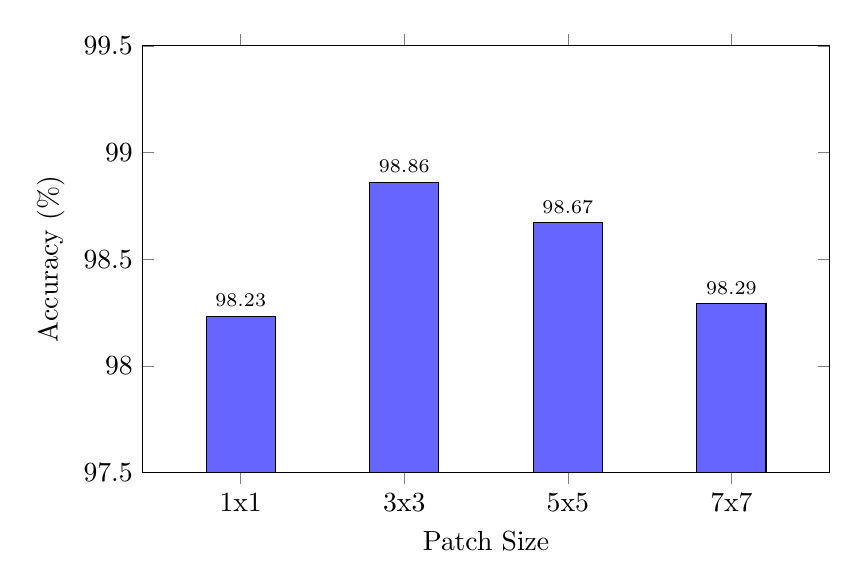
\begin{tikzpicture}
        \begin{axis}[
            ybar,
            width=0.85\textwidth,
            height=7cm,
            ylabel={Accuracy (\%)},
            xlabel={Patch Size},
            symbolic x coords={1x1, 3x3, 5x5, 7x7},
            xtick=data,
            ymin=97.5,
            ymax=99.5,
            bar width=25pt,
            nodes near coords,
            nodes near coords align={vertical},
            every node near coord/.append style={font=\scriptsize},
            enlarge x limits=0.2,
        ]
        \addplot[fill=blue!60] coordinates {
            (1x1, 98.23)
            (3x3, 98.86)
            (5x5, 98.67)
            (7x7, 98.29)
        };
        \end{axis}
    \end{tikzpicture}
    \caption{So sánh Accuracy theo các Patch Size}
    \label{fig:patch_size_comparison}
\end{figure}

\textbf{Kết luận}: \textbf{Patch size 3×3 là tối ưu} cho bộ dữ liệu này.

\subsection{Ảnh hưởng của nguồn dữ liệu}

\begin{table}[H]
\centering
\caption{Nghiên cứu loại trừ các nguồn dữ liệu (Ablation Study)}
\label{tab:data_sources}
\begin{tabular}{|l|c|c|c|}
\hline
\textbf{Configuration} & \textbf{Features} & \textbf{Accuracy} & \textbf{ROC-AUC} \\
\hline
Chỉ Sentinel-2 (trước) & 7 & 96.21\% & 98.95\% \\
\hline
Sentinel-2 (trước + sau + delta) & 21 & 98.48\% & 99.68\% \\
\hline
Chỉ Sentinel-1 (trước + sau + delta) & 6 & 94.19\% & 97.83\% \\
\hline
\textbf{S1 + S2 (tất cả)} & \textbf{27} & \textbf{98.86\%} & \textbf{99.98\%} \\
\hline
\end{tabular}
\end{table}

\begin{figure}[H]
    \centering
    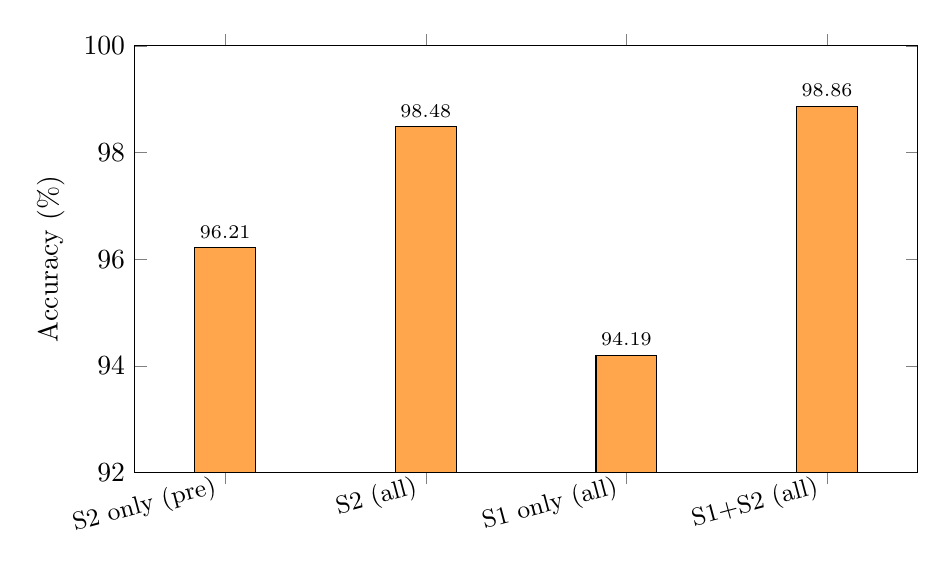
\begin{tikzpicture}
        \begin{axis}[
            ybar,
            width=0.95\textwidth,
            height=7cm,
            ylabel={Accuracy (\%)},
            symbolic x coords={S2 only (pre), S2 (all), S1 only (all), S1+S2 (all)},
            xtick=data,
            xticklabel style={rotate=15, anchor=east, font=\small},
            ymin=92,
            ymax=100,
            bar width=22pt,
            nodes near coords,
            nodes near coords align={vertical},
            every node near coord/.append style={font=\scriptsize},
            enlarge x limits=0.15,
        ]
        \addplot[fill=orange!70] coordinates {
            (S2 only (pre), 96.21)
            (S2 (all), 98.48)
            (S1 only (all), 94.19)
            (S1+S2 (all), 98.86)
        };
        \end{axis}
    \end{tikzpicture}
    \caption{So sánh Accuracy theo các nguồn dữ liệu}
    \label{fig:data_sources_comparison}
\end{figure}

\textbf{Kết luận}: \textbf{Kết hợp Sentinel-1 và Sentinel-2} cho kết quả tối ưu nhất, dữ liệu radar và quang học bổ sung cho nhau.